% ============================================================
\chapter{Signed Measures and Hahn-Jordan Decomposition}
\label{ch:signed_measures}
% ============================================================

\section{Introduction}

Until now, measures have been positive quantities: area, volume, probability. But physics and economics abound with quantities that change sign: an electric charge can be positive or negative, a financial balance can be profit or loss, the difference of two probability measures is no longer a positive measure. Johann Radon and Otton Nikodym, in the 1910s--1930s, showed that every signed measure decomposes canonically into a positive part and a negative part (Jordan decomposition), concentrated on disjoint sets (Hahn decomposition). The Radon--Nikodym theorem, which expresses an absolutely continuous measure with respect to another as a weighted integral, crowns this theory and provides the rigorous definition of the probability density function.

\begin{intuition}[title=\textbf{Why signed measures?}]
Consider an electric charge distribution on a surface: some regions carry positive
charge, others negative. The total ``charge measure'' of a set can be positive,
negative, or zero. This is exactly what a signed measure models. Moreover, the
difference of two (positive) finite measures is always a signed measure.
\end{intuition}

% ------------------------------------------------------------
\section{Definitions and first examples}
% ------------------------------------------------------------

\begin{definition}[Signed measure]
\label{def:signed_measure}
\index{signed measure}
Let $(X, \mathcal{A})$ be a measurable space. A \emph{signed measure} on
$(X, \mathcal{A})$ is a function $\nu : \mathcal{A} \to [-\infty, +\infty]$
satisfying:
\begin{enumerate}
    \item[(i)] $\nu(\varnothing) = 0$;
    \item[(ii)] $\nu$ assumes \emph{at most} one of the values $+\infty$ and $-\infty$;
    \item[(iii)] (\emph{$\sigma$-additivity}) for every sequence $(A_n)_{n \geq 1}$
    of mutually disjoint sets in $\mathcal{A}$:
    \[
        \nu\!\left(\bigcup_{n=1}^{\infty} A_n\right)
        = \sum_{n=1}^{\infty} \nu(A_n),
    \]
    where the series converges absolutely if the left-hand side is finite.
\end{enumerate}
\end{definition}

\begin{remark}
Condition (ii) is essential to avoid indeterminate expressions of the form
$+\infty - \infty$. Every positive measure is a signed measure (special case).
\end{remark}

\begin{example}
\begin{enumerate}
    \item If $\mu$ and $\lambda$ are positive measures on $(X, \mathcal{A})$ with
    $\lambda$ finite, then $\nu = \mu - \lambda$ is a signed measure.
    \item If $f \in L^1(\mu)$, then $\nu(A) = \int_A f\, d\mu$ is a finite signed
    measure.
\end{enumerate}
\end{example}

\begin{definition}[Positive, negative, and null sets]
Let $\nu$ be a signed measure on $(X, \mathcal{A})$.
\begin{itemize}
    \item A set $A \in \mathcal{A}$ is \emph{positive}\index{positive set} for $\nu$ if
    $\nu(B) \geq 0$ for every $B \in \mathcal{A}$ with $B \subset A$.
    \item A set $A$ is \emph{negative}\index{negative set} for $\nu$ if
    $\nu(B) \leq 0$ for every $B \in \mathcal{A}$ with $B \subset A$.
    \item A set $A$ is \emph{null}\index{null set} for $\nu$ if
    $\nu(B) = 0$ for every $B \in \mathcal{A}$ with $B \subset A$.
\end{itemize}
\end{definition}

\begin{attention}[title=\textbf{Positive for $\nu$ $\neq$ $\nu(A) \geq 0$}]
A set $A$ is positive for $\nu$ if \emph{all} its measurable subsets have nonnegative
signed measure. The fact that $\nu(A) \geq 0$ alone does not suffice: there may exist
$B \subset A$ with $\nu(B) < 0$.
\end{attention}

% ------------------------------------------------------------
\section{Hahn decomposition}
% ------------------------------------------------------------

\begin{lemma}
\label{lem:hahn_negative}
Let $\nu$ be a signed measure on $(X, \mathcal{A})$ and let $A \in \mathcal{A}$ with
$-\infty < \nu(A) < 0$. Then there exists a negative set $B \subset A$ with
$\nu(B) \leq \nu(A)$.
\end{lemma}

\begin{proof}
If $A$ is already negative, take $B = A$. Otherwise, there exists $A_1 \subset A$ with
$\nu(A_1) > 0$. Let $n_1$ be the smallest integer such that some measurable subset of
$A$ has $\nu$-value $\geq 1/n_1$. Iterate: in $A \setminus A_1$, find $A_2$ with
$\nu(A_2) \geq 1/n_2$, etc. Set $B = A \setminus \bigcup_k A_k$. Then
$\nu(B) = \nu(A) - \sum_k \nu(A_k) \leq \nu(A)$, and
$\sum_k 1/n_k < \infty$, so $1/n_k \to 0$. If $C \subset B$ had $\nu(C) > 0$,
we could find $n$ with $\nu(C) \geq 1/n$, contradicting the choice of $n_k$
when $1/n_k < 1/n$. Hence $B$ is negative.
\end{proof}

% Hahn decomposition diagram
\begin{center}
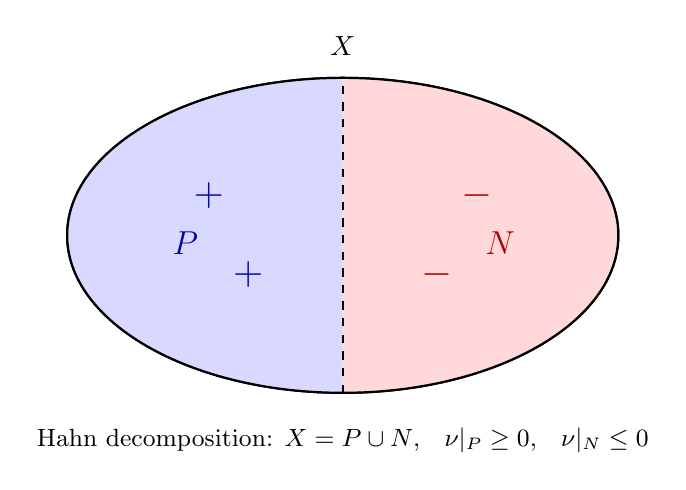
\begin{tikzpicture}[scale=1.0]
  % Set X (outer ellipse)
  \draw[thick] (0,0) ellipse (3.5cm and 2cm);
  \node at (0,2.4) {$X$};
  % Separating line
  \draw[thick, dashed] (0,-2) -- (0,2);
  % Region P (positive, blue)
  \fill[blue!15] (0,0) -- (0,2) arc[start angle=90, end angle=270,
    x radius=3.5cm, y radius=2cm] -- cycle;
  % Region N (negative, red)
  \fill[red!15] (0,0) -- (0,2) arc[start angle=90, end angle=-90,
    x radius=3.5cm, y radius=2cm] -- cycle;
  % Redraw outline and separator
  \draw[thick] (0,0) ellipse (3.5cm and 2cm);
  \draw[thick, dashed] (0,-2) -- (0,2);
  % Labels and signs
  \node[blue!70!black, font=\Large\bfseries] at (-1.7,0.5) {$+$};
  \node[blue!70!black, font=\Large\bfseries] at (-1.2,-0.5) {$+$};
  \node[red!70!black, font=\Large\bfseries] at (1.7,0.5) {$-$};
  \node[red!70!black, font=\Large\bfseries] at (1.2,-0.5) {$-$};
  \node[blue!70!black, font=\large] at (-2.0,-0.1) {$P$};
  \node[red!70!black, font=\large] at (2.0,-0.1) {$N$};
  % Caption
  \node at (0,-2.6) {\small Hahn decomposition: $X = P \cup N$, \;
    $\nu|_P \geq 0$, \; $\nu|_N \leq 0$};
\end{tikzpicture}
\end{center}

\begin{theorem}[Hahn Decomposition]
\label{thm:hahn}
\index{Hahn decomposition}
Let $\nu$ be a signed measure on $(X, \mathcal{A})$. There exists a partition
$X = P \cup N$ with $P, N \in \mathcal{A}$, $P \cap N = \varnothing$, such that
$P$ is a positive set and $N$ is a negative set for $\nu$.

Moreover, this decomposition is \emph{essentially unique}: if $X = P' \cup N'$ is
another Hahn decomposition, then $P \triangle P'$ (and $N \triangle N'$) is a null
set for $\nu$.
\end{theorem}

\begin{proof}
Assume $\nu$ does not take the value $+\infty$ (the symmetric case is analogous).
Let $\lambda = \inf\{\nu(A) : A \in \mathcal{A}\} \in [-\infty, 0]$. For each
$n \geq 1$, choose $A_n$ with $\nu(A_n) < \lambda + 1/n$. By
Lemma~\ref{lem:hahn_negative}, there exists a negative set $B_n \subset A_n$ with
$\nu(B_n) \leq \nu(A_n)$.

Set $N = \bigcup_n B_n$. As a countable union of negative sets, $N$ is negative.
Moreover, $\nu(N) \leq \nu(B_n) < \lambda + 1/n$ for all $n$, so $\nu(N) = \lambda$.
Set $P = X \setminus N$. If $P$ were not positive, there would exist $A \subset P$
with $\nu(A) < 0$, yielding a negative subset $B \subset A$ with
$\nu(N \cup B) = \nu(N) + \nu(B) < \lambda$, a contradiction.

For essential uniqueness: $P \cap N' \subset P$ (positive) and $P \cap N' \subset N'$
(negative), so $P \cap N'$ is null. Similarly $P' \cap N$ is null.
\end{proof}

% ------------------------------------------------------------
\section{Jordan decomposition and total variation}
% ------------------------------------------------------------

\begin{definition}[Jordan decomposition]
\label{def:jordan}
\index{Jordan decomposition}
Let $\nu$ be a signed measure and $X = P \cup N$ a Hahn decomposition. The
\emph{positive and negative parts} of $\nu$ are:
\[
    \nu^+(A) = \nu(A \cap P), \qquad \nu^-(A) = -\nu(A \cap N),
\]
for all $A \in \mathcal{A}$. Then $\nu = \nu^+ - \nu^-$.
\end{definition}

\begin{theorem}[Jordan Decomposition]
The measures $\nu^+$ and $\nu^-$ are positive measures on $(X, \mathcal{A})$, at
least one of them is finite, and they do not depend on the choice of Hahn
decomposition. Moreover, $\nu^+ \perp \nu^-$ (mutual singularity).
\end{theorem}

\begin{definition}[Total variation]
\label{def:total_variation}
\index{total variation}
The \emph{total variation} of $\nu$ is the positive measure:
\[
    \abs{\nu} = \nu^+ + \nu^-.
\]
The \emph{total variation of $\nu$ on $X$} is $\norm{\nu} = \abs{\nu}(X)$.
\end{definition}

\begin{proposition}[Properties of total variation]
For any signed measure $\nu$ and any $A \in \mathcal{A}$:
\begin{enumerate}
    \item $\abs{\nu(A)} \leq \abs{\nu}(A)$;
    \item $\abs{\nu}(A) = \sup\bigl\{\sum_{i=1}^n \abs{\nu(A_i)} :
    A = \bigsqcup_{i=1}^n A_i,\, A_i \in \mathcal{A}\bigr\}$;
    \item $\nu$ is a finite signed measure if and only if $\abs{\nu}(X) < \infty$.
\end{enumerate}
\end{proposition}

\begin{proof}
(1) $\abs{\nu(A)} = \abs{\nu^+(A) - \nu^-(A)} \leq \nu^+(A) + \nu^-(A) = \abs{\nu}(A)$.

(2) For any partition $A = \bigsqcup_i A_i$,
$\sum_i \abs{\nu(A_i)} \leq \sum_i \abs{\nu}(A_i) = \abs{\nu}(A)$.
The reverse inequality follows by taking the partition $A = (A \cap P) \sqcup (A \cap N)$.

(3) Immediate since $\norm{\nu} = \nu^+(X) + \nu^-(X)$.
\end{proof}

\begin{keyformulas}[title=\textbf{Summary: Jordan decomposition}]
For any signed measure $\nu$:
\begin{align*}
    \nu &= \nu^+ - \nu^-, \qquad \abs{\nu} = \nu^+ + \nu^-, \\
    \nu^+ &= \frac{\abs{\nu} + \nu}{2}, \qquad
    \nu^- = \frac{\abs{\nu} - \nu}{2}.
\end{align*}
\end{keyformulas}

% ------------------------------------------------------------
\section{Mutual singularity}
% ------------------------------------------------------------

\begin{definition}[Mutually singular measures]
\index{mutually singular measures}
Two signed measures $\mu$ and $\nu$ on $(X, \mathcal{A})$ are \emph{mutually
singular}, written $\mu \perp \nu$, if there exists a partition $X = A \cup B$
with $A, B \in \mathcal{A}$ such that $\abs{\mu}(B) = 0$ and $\abs{\nu}(A) = 0$.
\end{definition}

\begin{example}
\begin{enumerate}
    \item Lebesgue measure $\lambda$ on $\R$ and the Dirac measure $\delta_0$ are
    mutually singular: $\lambda(\{0\}) = 0$ and $\delta_0(\R \setminus \{0\}) = 0$.
    \item Lebesgue measure and the Cantor--Vitali measure on $[0,1]$ are mutually
    singular.
\end{enumerate}
\end{example}

% ------------------------------------------------------------
\section{The Banach space of finite signed measures}
% ------------------------------------------------------------

\begin{proposition}
The set $\mathcal{M}(X, \mathcal{A})$ of finite signed measures on
$(X, \mathcal{A})$ is a real vector space, and $\norm{\nu} = \abs{\nu}(X)$ is a
norm. Moreover, $(\mathcal{M}(X, \mathcal{A}), \norm{\cdot})$ is a Banach space.
\end{proposition}

% ------------------------------------------------------------
\section{Exercises}
% ------------------------------------------------------------

\begin{exercise}
Let $\nu$ be a finite signed measure on $(X, \mathcal{A})$. Show that $\nu$ is
bounded, i.e.\ $\sup_{A \in \mathcal{A}} \abs{\nu(A)} < \infty$.
\end{exercise}

\begin{exercise}
Let $f \in L^1(\R, \lambda)$ where $\lambda$ is Lebesgue measure. Show that
$\nu(A) = \int_A f\, d\lambda$ defines a signed measure and compute $\nu^+$,
$\nu^-$, $\abs{\nu}$ in terms of $f$.
\emph{Hint}: show that $\nu^+(A) = \int_A f^+\, d\lambda$ and
$\nu^-(A) = \int_A f^-\, d\lambda$.
\end{exercise}

\begin{exercise}
Show that two positive measures $\mu$ and $\nu$ are mutually singular if and only
if $\inf_{A \in \mathcal{A}} [\mu(A) + \nu(A^c)] = 0$.
\end{exercise}

\begin{exercise}
Let $\nu$ be a signed measure and $(A_n)$ an increasing sequence in $\mathcal{A}$.
Show that $\nu(\bigcup_n A_n) = \lim_n \nu(A_n)$ (monotone continuity for signed
measures).
\end{exercise}

\begin{exercise}[Explicit Hahn decomposition]
Let $\nu$ be the signed measure on $(\R, \mathcal{B}(\R))$ defined by
$\nu(A) = \int_A (x^2 - 1) e^{-x^2}\, d\lambda(x)$. Find a Hahn decomposition
of $\R$ for $\nu$ and deduce $\nu^+$, $\nu^-$.
\end{exercise}

\begin{exercise}
Let $\nu$ be a finite signed measure. Show that for every $\varepsilon > 0$, the
collection $\{A \in \mathcal{A} : \abs{\nu(A)} > \varepsilon\}$ is finite.
\emph{Hint}: use $\abs{\nu}(X) < \infty$.
\end{exercise}
